\section{Proposed Model}
\label{sec:method}

The proposed model, CardioSentinel, classifies a 10-s, 12-lead ECG into the five PTB-XL diagnostic
superclasses with a privacy-preserving, one-shot federated scheme. The training records are divided
into four disjoint, patient-separated partitions that play the role of four institutions. Each
client preprocesses its own recordings identically, trains its own network architecture locally,
and calibrates it with a single temperature. The central server never receives signals or
parameters; it receives only the calibrated class probabilities of the clients and combines them
with weights constrained to the probability simplex. The weighting rule, the per-class decision
thresholds and an optional triage band are all fitted on a separate validation fold, and the
combined prediction is explained with Integrated Gradients and with Shapley values over clients.
The six subsections below describe the architecture, the preprocessing, the features, the
classification task, the federated protocol and the explainability methods.

% ---------------------------------------------------------------------------------- A
\subsection{Architecture}
\label{sec:arch}

Fig.~\ref{fig:arch} shows the architecture. The \emph{data} block at the bottom holds the PTB-XL
records, already split by the official stratified folds into four client partitions, a validation
fold and a test fold. The \emph{pre-processing} block applies the same signal pipeline at every
client (Section~\ref{sec:prep}). The \emph{feature analysis} stage is performed inside each client
network, which learns its own representation of the 12 leads (Section~\ref{sec:features}). Each of
the four \emph{local client models} ends in its own classifier head, marked C in the figure, that
outputs five logits; these are converted into calibrated probabilities with a per-client
temperature. The \emph{federated server} combines the four probability vectors with the simplex
weights $w_i$ into the \emph{global model} output, the \emph{classification} block turns the global
probabilities into five binary decisions with per-class thresholds and, optionally, into
automatic-or-referred triage decisions, and the \emph{explainability} block attributes the global
output to leads and time.

\begin{figure*}[!t]
\centering
\resizebox{\textwidth}{!}{%
\begin{tikzpicture}[
  font=\footnotesize, >={Stealth[length=2mm]},
  box/.style={draw, rounded corners=2pt, align=center, minimum height=0.85cm, fill=#1},
  box/.default=white,
  lab/.style={font=\scriptsize\itshape, text=black!65}]
  % data (bottom)
  \node[box=blue!6, minimum width=19cm, minimum height=1.0cm] (data) at (0,0) {};
  \node[anchor=west, font=\footnotesize\bfseries, align=left] at (-9.4,0) {Data:\\PTB-XL};
  \node[draw, fill=white, minimum width=2.2cm, minimum height=0.65cm, align=center, font=\scriptsize] at (-6.5,0) {Folds 1--2\\(4,277 ECGs)};
  \node[draw, fill=white, minimum width=2.2cm, minimum height=0.65cm, align=center, font=\scriptsize] at (-3.9,0) {Folds 3--4\\(4,280)};
  \node[draw, fill=white, minimum width=2.2cm, minimum height=0.65cm, align=center, font=\scriptsize] at (-1.3,0) {Folds 5--6\\(4,264)};
  \node[draw, fill=white, minimum width=2.2cm, minimum height=0.65cm, align=center, font=\scriptsize] at (1.3,0) {Folds 7--8\\(4,263)};
  \node[draw, fill=white, minimum width=2.6cm, minimum height=0.65cm, align=center, font=\scriptsize] at (4.6,0) {Fold 9: validation\\(2,146, server)};
  \node[draw, fill=white, minimum width=2.6cm, minimum height=0.65cm, align=center, font=\scriptsize] at (7.6,0) {Fold 10: test\\(2,158, held out)};
  % preprocessing
  \node[box=orange!8, minimum width=19cm, text width=18.6cm] (prep) at (0,1.5)
    {\textbf{Pre-processing (identical at every client):} lead reordering $\rightarrow$ NaN removal $\rightarrow$
     crop/pad to 1,000 samples $\rightarrow$ 0.5--40 Hz Butterworth band-pass $\rightarrow$ per-lead z-score, clip $\pm10$
     $\rightarrow$ train-only augmentation};
  \draw[->] (data) -- (prep);
  \node[lab, anchor=west] at (-9.5,2.35) {Local client models (private data, own architecture)};
  % clients
  \foreach \x/\c/\a/\f in {-6.5/A/{1D CNN\\4 conv blocks}/{$h_A\in\mathbb{R}^{512}$},
                           -2.2/B/{1D ResNet\\16 residual blocks}/{$h_B\in\mathbb{R}^{256}$},
                            2.1/C/{BiLSTM\\2 layers, 128 units}/{$h_C\in\mathbb{R}^{512}$},
                            6.4/D/{CNN-LSTM\\3 conv + BiLSTM}/{$h_D\in\mathbb{R}^{512}$}} {
    \node[box=green!7, minimum width=3.2cm] (m\c) at (\x,3.2) {\textbf{Client \c}: \a};
    \node[box=green!3, minimum width=3.2cm, minimum height=0.6cm] (f\c) at (\x,4.45) {Local features \f};
    \node[draw, circle, fill=yellow!25, minimum size=0.75cm, font=\footnotesize\bfseries] (c\c) at (\x,5.55) {C};
    \node[anchor=west, font=\scriptsize, align=left] at (\x+0.45,5.55) {head + $T_\c$\\$P_\c(y\mid x)$};
    \draw[->] (\x,1.95) -- (m\c);
    \draw[->] (m\c) -- (f\c);
    \draw[->] (f\c) -- (c\c);
    \draw[->] (c\c) -- (\x,6.65);
  }
  % server
  \node[box=red!7, minimum width=19cm] (gate) at (0,7.1)
    {\textbf{Federated server: weighted gate} \quad $P(y\mid x)=\sum_{i} w_i\,P_i(y\mid x)$, \; $w\in\Delta^{3}$ \quad
     (equal / static / dynamic weights, selected by patient-grouped CV on fold 9)};
  \node[box=red!3, minimum width=7.5cm] (out) at (-4.5,8.55)
    {\textbf{Global output:} 5 calibrated probabilities\\$\rightarrow$ per-class thresholds $\tau_c$ (multi-label)};
  \node[box=violet!7, minimum width=7.5cm] (xai) at (4.5,8.55)
    {\textbf{Explainability:} Integrated Gradients per lead/time;\\Shapley value per client};
  \draw[->] (-4.5,7.55) -- (out);
  \draw[->] (4.5,7.55) -- (xai);
  \node[box=gray!8, minimum width=7.5cm, text width=7.3cm] (tri) at (-4.5,10.0)
    {\textbf{Classification / triage:} rule in ($p\ge h_c$), rule out ($p\le l_c$), otherwise refer to a cardiologist};
  \draw[->] (out) -- (tri);
\end{tikzpicture}}
\caption{Architecture of the proposed CardioSentinel model. Four clients hold disjoint, patient-separated
PTB-XL partitions, apply the same pre-processing, learn their own features with different network
architectures and expose only calibrated probabilities through their classifier heads (C). The
server combines the probabilities on the simplex, thresholds them per class and explains the global
output.}
\label{fig:arch}
\end{figure*}

\textit{Model progression.} The four clients were deliberately chosen to span the main families of
ECG networks, from purely convolutional to purely recurrent, so that their errors are as diverse as
possible. Client~A is a plain 1D CNN with four blocks of a 7-tap convolution (no bias), batch
normalisation, ReLU and max-pooling by two, with 32, 64, 128 and 256 channels. For an input
$x\in\mathbb{R}^{12\times 1000}$ each block computes
\begin{equation}
  h^{(l+1)} = \mathrm{MaxPool}_2\big(\mathrm{ReLU}(\mathrm{BN}(W^{(l)} * h^{(l)}))\big),
\end{equation}
and the final feature map is summarised by concatenated global average and global max pooling,
$\mathrm{AM}(h)=[\tfrac{1}{T}\sum_t h_t;\,\max_t h_t]$. Client~B is a 1D ResNet \cite{he2016resnet}
with a 7-tap, 64-channel stem and stages of 64, 128, 256 and 256 channels containing 3, 4, 6 and 3
residual blocks with 5-tap kernels, in which the last batch normalisation of each block is
initialised to zero so that each block starts as the identity, $h^{(l+1)}=\mathrm{ReLU}(F(h^{(l)})+S(h^{(l)}))$.
Client~C is a two-layer bidirectional LSTM \cite{hochreiter1997lstm,schuster1997bilstm} with 128
hidden units per direction that reads the 1,000 time steps directly; each direction updates
\begin{align}
  i_t &= \sigma(W_i x_t + U_i h_{t-1} + b_i), \nonumber\\
  f_t &= \sigma(W_f x_t + U_f h_{t-1} + b_f), \nonumber\\
  o_t &= \sigma(W_o x_t + U_o h_{t-1} + b_o), \nonumber\\
  g_t &= \tanh(W_c x_t + U_c h_{t-1} + b_c), \nonumber\\
  c_t &= f_t\odot c_{t-1} + i_t\odot g_t, \qquad h_t = o_t\odot\tanh(c_t),
\end{align}
and the forward and backward states are concatenated and pooled with $\mathrm{AM}(\cdot)$. Client~D is
a CNN-LSTM hybrid in which three convolutional blocks (32, 64 and 128 channels) shorten the sequence
from 1,000 to 125 steps before a one-layer BiLSTM with 128 hidden units, so that local wave
morphology is captured by the convolutions and rhythm context by the recurrence. All clients share
the same head, $\mathrm{Linear}(d\!\rightarrow\!256)\!\rightarrow\!\mathrm{ReLU}\!\rightarrow\!
\mathrm{Dropout}(0.3)\!\rightarrow\!\mathrm{Linear}(256\!\rightarrow\!5)$, and the same training
recipe, so that only the architecture and the data differ. On the held-out test fold this
progression moves the macro AUROC from 0.882--0.888 for the convolutional clients to 0.894 for the
BiLSTM and 0.896 for the CNN-LSTM, and the federated gate over all four reaches 0.905
(Section~\ref{sec:comparison}). An attention-based client was not part of the study.

Algorithm~\ref{alg:cardiomoe} summarises the complete method, from preprocessing to the explained,
triaged prediction.

\begin{algorithm}[!t]
\caption{CardioSentinel: one-shot federated classification of 12-lead ECGs}
\label{alg:cardiomoe}
\footnotesize
\begin{algorithmic}[1]
\Require Client partitions $\mathcal{D}_A,\dots,\mathcal{D}_D$ (folds 1--8), validation fold $\mathcal{V}$ (fold 9), test ECG $x$
\Ensure Calibrated probabilities $P(y\mid x)$, multi-label decision $y^{\mathrm{pred}}$, triage status, attributions
\For{each client $i\in\{A,B,C,D\}$ \textbf{in parallel}} \Comment{local, private}
  \State Pre-process every record of $\mathcal{D}_i$ (band-pass, z-score, clip)
  \State Train network $f_i$ with weighted BCE, AdamW and OneCycle; early-stop on macro AUROC of $\mathcal{V}$
  \State Fit temperature $T_i$ on $\mathcal{V}$; $P_i(y\mid x)\gets\sigma(f_i(x)/T_i)$
\EndFor
\State Server collects $P_i(y\mid v)$ for all $v\in\mathcal{V}$ \Comment{probabilities only}
\For{combiner $g\in(\text{equal},\text{static},\text{dynamic})$}
  \State Obtain out-of-fold predictions by patient-grouped 5-fold CV on $\mathcal{V}$; record macro AUROC $a_g$
\EndFor
\State $g^\star\gets$ equal; \textbf{for} $g$ in (static, dynamic): \textbf{if} $a_g\ge a_{g^\star}+0.002$ \textbf{then} $g^\star\gets g$
\State Refit $g^\star$ on $\mathcal{V}$; tune per-class thresholds $\tau_c$ and triage bands $(l_c,h_c)$ on its CV predictions
\State \textbf{Inference:} $P(y\mid x)\gets\sum_i w_i^{g^\star}(x)\,P_i(y\mid x)$; $y^{\mathrm{pred}}_c\gets[P(y_c\mid x)\ge\tau_c]$
\State Triage: rule in if $P(y_c\mid x)\ge h_c$, rule out if $\le l_c$, else refer
\State Explain $P(y_c\mid x)$ with Integrated Gradients over leads and time
\end{algorithmic}
\end{algorithm}

% ---------------------------------------------------------------------------------- B
\subsection{Preprocessing}
\label{sec:prep}

All preprocessing steps are listed in Table~\ref{tab:prep}. They are implemented once and executed
identically by every client, so no client-specific normalisation statistics are needed and no
information crosses client boundaries.

\textit{Label encoding and cleaning.} Each record's SCP-ECG statements are mapped to the
\texttt{diagnostic\_class} column of \texttt{scp\_statements.csv}, keeping only the 44 statements
flagged as diagnostic, and encoded as a multi-hot vector over (NORM, MI, STTC, CD, HYP). Records
without any diagnostic superclass cannot be labelled and are removed, which reduces the 21,799
records to 21,388. No other record is excluded.

\textit{Signal cleaning.} The 100-Hz waveforms are read with the WFDB library and reordered to I,
II, III, aVR, aVL, aVF, V1--V6, matching lead names case-insensitively. Non-finite samples are
replaced by zero, and every signal is cropped or zero-padded to exactly 1,000 samples. Baseline
wander and high-frequency noise are removed with a third-order Butterworth band-pass filter between
0.5 and 40~Hz applied forwards and backwards, so that the filter introduces no phase shift. The
filtered signals are stored in millivolts without normalisation.

\textit{Normalisation.} At load time each lead of each recording is z-scored with its own mean and
standard deviation, $x^{\mathrm{norm}}_{\ell t}=(x_{\ell t}-\mu_\ell)/\sigma_\ell$, clipped to $[-10,10]$, and a
lead whose standard deviation is below $10^{-6}$ is set to zero. Because the statistics are
per-recording, the normalisation needs no shared population statistics, which is essential in the
federated setting.

\textit{Augmentation and class balancing.} During training only, each signal is multiplied by a
random amplitude factor in $[0.9,1.1]$, white Gaussian noise is added at a signal-to-noise ratio
drawn from 20--30~dB, a sinusoidal baseline wander of 0.1--0.5~Hz with an amplitude of 0.05--0.3
standard deviations is added to every lead, and each lead is zeroed with probability 0.05. Class
imbalance is handled in the loss rather than by resampling: the positive term of each class is
weighted by the ratio of negatives to positives in the client's training data
(Section~\ref{sec:clf}). Modality alignment is not required because a single modality is used, but
all leads are aligned in time by construction.

\begin{table}[!t]
\centering
\caption{Pre-processing steps and parameters}
\label{tab:prep}
\footnotesize
\begin{tabular}{@{}p{2.1cm}p{5.9cm}@{}}
\toprule
Step & Method and parameters \\
\midrule
Label encoding & SCP codes $\rightarrow$ 5 diagnostic superclasses (44 diagnostic statements); multi-hot \\
Record cleaning & Remove records without a superclass (21,799 $\rightarrow$ 21,388) \\
Lead order & I, II, III, aVR, aVL, aVF, V1--V6 \\
Missing values & NaN/$\pm\infty$ $\rightarrow$ 0 \\
Length & 100 Hz, crop/zero-pad to 1,000 samples (10 s) \\
Filtering & Butterworth band-pass 0.5--40 Hz, order 3, zero-phase \\
Normalisation & Per-lead, per-record z-score; clip to $\pm10$; flat lead $\rightarrow$ 0 \\
Augmentation (train) & Amplitude $\times\mathcal{U}(0.9,1.1)$; noise SNR $\mathcal{U}(20,30)$ dB; wander 0.1--0.5 Hz, amp.\ $\mathcal{U}(0.05,0.3)$; lead dropout $p=0.05$ \\
Class balancing & BCE positive weight $=\#\text{neg}/\#\text{pos}$ per class \\
\bottomrule
\end{tabular}
\end{table}

% ---------------------------------------------------------------------------------- C
\subsection{Feature Analysis}
\label{sec:features}

No hand-crafted features are extracted. Every client learns its features end-to-end from the
normalised 12-lead signal, and the four architectures look at the signal in complementary ways, as
summarised in Table~\ref{tab:features}. The convolutional clients extract local morphological
features (QRS complexes, ST segments and T waves) whose receptive field grows with depth; the BiLSTM
integrates the whole 10-s recording in both directions and is sensitive to rhythm and to the
temporal relation between beats; the CNN-LSTM first compresses local morphology into 125 steps and
then models their sequence. All clients summarise the time axis with concatenated average and max
pooling, which preserves both the typical and the most extreme activation of each feature channel.

The correlation structure of the input explains why a lead-wise model is appropriate. The 12 leads
are not independent: the limb leads are linear combinations of two measured potentials, and
neighbouring precordial leads view the heart from similar angles. Fig.~\ref{fig:leadcorr} shows the
mean Pearson correlation between the normalised leads over 17,083 training recordings (one recording
with a flat lead was skipped). The leads facing the left ventricle form one strongly correlated group:
I, II, V4, V5 and V6 correlate with each other at $r=0.62$--$0.92$, and aVR mirrors them
($r=-0.69$ to $-0.90$). The inferior leads III and aVF form a second group ($r=0.74$), anti-correlated
with aVL ($r=-0.72$ for III), whereas the right precordial leads V1--V3 are only weakly related to the
lateral group (for example $r=0.02$ between V2 and V5). Much of the 12-lead input is therefore
redundant, while V1--V3 and the inferior leads carry largely separate information. Feature selection
is left to the networks, and lead dropout during training discourages them from relying on a single
lead.

Fusion is performed at the decision level. Feature-level fusion of the client embeddings
$h_i$ would require the clients to transmit internal representations of every patient and to agree
on a common embedding space, which both weakens privacy and is not meaningful for networks of
different design. Each client therefore maps its own features to calibrated class probabilities, and
only these are fused (Section~\ref{sec:fl}).

\begin{table}[!t]
\centering
\caption{Learned features per client}
\label{tab:features}
\footnotesize
\setlength{\tabcolsep}{3pt}
\resizebox{\columnwidth}{!}{%
\begin{tabular}{@{}llcl@{}}
\toprule
Client & Feature extractor & Pooled dim. & Main signal property \\
\midrule
A & 4 conv blocks, k=7, 32--256 ch. & 512 & Local wave morphology \\
B & ResNet, 16 blocks, k=5, 64--256 ch. & 512$\rightarrow$256 & Hierarchical morphology \\
C & 2-layer BiLSTM, 128 units, 1,000 steps & 512 & Rhythm, beat-to-beat context \\
D & 3 conv blocks + BiLSTM, 125 steps & 512 & Morphology and rhythm \\
\bottomrule
\end{tabular}}
\end{table}

\begin{figure}[!t]
\centering
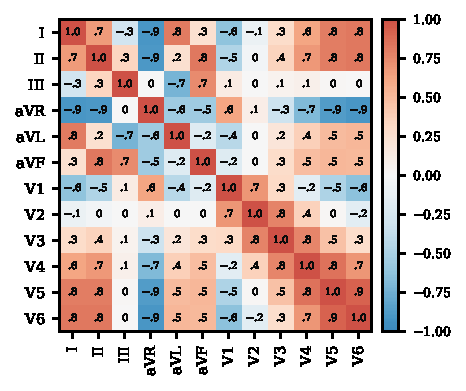
\includegraphics[width=0.85\columnwidth]{lead_corr}
\caption{Mean Pearson correlation between the 12 normalised leads over the training folds 1--8.}
\label{fig:leadcorr}
\end{figure}

% ---------------------------------------------------------------------------------- D
\subsection{Classification and Regression}
\label{sec:clf}

\textit{Classification.} The task is multi-label: a recording can belong to several superclasses at
once, and in PTB-XL 24.1\% of the retained records carry more than one superclass. The output layer
of each client therefore has five independent logits $z_{ic}$, and a sigmoid rather than a softmax
gives the class probabilities. Each client minimises the class-weighted binary cross-entropy
\begin{equation}
\begin{split}
\mathcal{L}_i = -\frac{1}{5N}\sum_{n=1}^{N}\sum_{c=1}^{5}\Big[&\beta_c\,y_{nc}\log\sigma(z_{nc})\\
 &+ (1-y_{nc})\log\big(1-\sigma(z_{nc})\big)\Big],
\end{split}
\end{equation}
with $\beta_c=N^{-}_c/N^{+}_c$ computed from the client's own training labels. After training, a
single temperature $T_i$ is fitted on the validation fold by minimising the same loss without
weights over $\sigma(z/T_i)$ \cite{guo2017calibration}, which rescales the confidence of the client
without changing its ranking. The final binary decision for class $c$ is
$y^{\mathrm{pred}}_c=[P(y_c\mid x)\ge\tau_c]$, where $\tau_c$ is the threshold that maximises the F1-score of
class $c$ on the validation predictions.

\textit{Regression.} The PTB-XL superclass task does not provide a continuous target such as a
severity score, so no regression head was trained and no regression metric (MAE, RMSE, $R^2$) is
reported. The only continuous quantities produced by the model are the calibrated probabilities,
which are used as graded risk scores by the triage rule: for each class a rule-in threshold $h_c$
and a rule-out threshold $l_c$ are fitted on validation data, findings with $l_c<P<h_c$ are referred
to a cardiologist, and coverage is always reported together with the precision and recall of the
automatically decided findings.

% ---------------------------------------------------------------------------------- E
\subsection{Federated Learning}
\label{sec:fl}

\textit{Clients and data split.} The $K=4$ clients receive the official PTB-XL training folds in
pairs: A folds 1--2, B folds 3--4, C folds 5--6 and D folds 7--8, i.e.\ about 4,270 records each. The
folds were constructed by the dataset authors so that all records of a patient lie in one fold and
the label distribution is similar across folds \cite{wagner2020ptbxl}; the partition is therefore
patient-disjoint and approximately IID with respect to the labels, and the heterogeneity of the
federation lies in the models: every client trains a different architecture with a different number
of parameters (0.44M to 6.73M). Fold 9 is held by the server as a validation set, and fold 10 is the
untouched test set.

\textit{Local training and communication.} Each client trains once, for up to 50 local epochs with
early stopping, and then fits its temperature. Federation therefore takes a single round: there is
no repeated exchange of parameters and no synchronisation between clients during training. At
fitting and inference time the server sends an ECG to the clients and receives one calibrated
5-dimensional probability vector from each, i.e.\ 20 numbers per ECG. In the experiments reported
here all parties were simulated on one machine, but no step of the method requires a client to
reveal its data, parameters or architecture. Fig.~\ref{fig:flow} shows the workflow and
Algorithm~\ref{alg:fl} the protocol.

\textit{Aggregation rule.} Parameter-averaging methods such as FedAvg \cite{mcmahan2017fedavg} update
a shared model as $\theta_{t+1}=\sum_{k=1}^{K}\frac{n_k}{n}\theta_k^{t+1}$, which is only defined
when all clients share the same parameter space. CardioSentinel instead aggregates the calibrated
predictions,
\begin{equation}
\label{eq:gate}
\begin{split}
P(y\mid x)&=\sum_{i=1}^{K} w_i(x)\,P_i(y\mid x),\\
w_i(x)&\ge 0,\qquad \sum_{i=1}^{K} w_i(x)=1,
\end{split}
\end{equation}
with the weights parameterised by a softmax so that the simplex constraint holds by construction.
This prediction-level aggregation is related to one-shot FL with ensembles of local models
\cite{guha2019oneshot} and to distillation-based schemes that also admit heterogeneous client models
\cite{li2019fedmd,lin2020feddf}; unlike the latter, it needs neither a public transfer dataset nor a
distillation step, because the calibrated mixture itself is the global model.
Three combiners of increasing complexity are considered. \emph{Equal weights} use $w_i=1/K$ and learn
nothing. \emph{Static weights} learn one global logit per client, $w=\mathrm{softmax}(\theta)$, by
minimising the binary cross-entropy of $P(y\mid x)$ on the validation data with full-batch Adam
(learning rate 0.05, 500 steps). The \emph{dynamic gate} is a per-patient mixture of experts
\cite{jacobs1991moe}: an MLP takes the 20 client probabilities and the four mean binary entropies
$H_i=-\frac{1}{5}\sum_c[p_{ic}\log p_{ic}+(1-p_{ic})\log(1-p_{ic})]$, passes them through a 32-unit
ReLU layer with dropout 0.2 and outputs $w(x)=\mathrm{softmax}(\cdot)$; its last layer is
initialised to zero so that it starts from equal weights, and it is trained with AdamW and early
stopping on a patient-grouped 20\% inner hold-out. All three are evaluated by patient-grouped
five-fold cross-validation inside the validation fold, and the selection rule of
Algorithm~\ref{alg:cardiomoe} adopts a more complex combiner only if its cross-validated macro AUROC
exceeds that of the current choice by at least 0.002. This rule was fixed before the multi-seed test
evaluation.

\textit{Privacy benefit.} Raw ECGs, patient identifiers, model parameters, gradients and internal
embeddings never leave a client. The server observes only five calibrated probabilities per client
and ECG, which is the information a clinical decision-support service would return anyway. The
scheme does not by itself provide formal guarantees such as differential privacy, and the server
must hold a labelled validation set to fit the gate.

\begin{figure}[!t]
\centering
\resizebox{\columnwidth}{!}{%
\begin{tikzpicture}[font=\scriptsize, >={Stealth[length=1.6mm]},
  cl/.style={draw, rounded corners=2pt, fill=green!7, minimum width=1.5cm, minimum height=1.0cm, align=center},
  sv/.style={draw, rounded corners=2pt, fill=red!7, minimum width=7.6cm, minimum height=0.9cm, align=center}]
  \node[sv] (srv) at (0,2.7) {\textbf{Server}: holds fold 9; fits gate $w$, thresholds $\tau_c$, triage bands\\
    receives only $P_i(y\mid x)\in[0,1]^5$ from each client};
  \foreach \x/\c/\a in {-2.85/A/1D CNN, -0.95/B/1D ResNet, 0.95/C/BiLSTM, 2.85/D/CNN-LSTM} {
    \node[cl] (k\c) at (\x,0) {\textbf{Client \c}\\\a\\private folds};
    \draw[->, thick, black!60] ($(k\c.north)+(-0.25,0)$) -- node[left, font=\tiny, align=right]{$P_\c$} ($(srv.south -| k\c.north)+(-0.25,0)$);
    \draw[<-, black!40, dashed] ($(k\c.north)+(0.25,0)$) -- node[right, font=\tiny]{$x$} ($(srv.south -| k\c.north)+(0.25,0)$);
  }
  \node[font=\tiny, align=center, text=black!60] at (0,-0.95)
    {\textbf{Step 1} (once): local training + temperature \quad \textbf{Step 2}: query $x$ $\rightarrow$ return calibrated $P_i$\quad
     \textbf{Step 3}: server mixes $\sum_i w_iP_i$};
\end{tikzpicture}}
\caption{Federated workflow. Clients train once on private data; afterwards the server sends an ECG
$x$ (dashed) and receives calibrated probabilities (solid). No parameters or raw training data are
exchanged.}
\label{fig:flow}
\end{figure}

\begin{algorithm}[!t]
\caption{One-shot federated protocol and gate selection}
\label{alg:fl}
\footnotesize
\begin{algorithmic}[1]
\Require $K=4$ clients with private data $\mathcal{D}_i$; server validation set $\mathcal{V}$ with patient IDs
\State \textbf{Round 1 (only round):} each client trains $f_i$ on $\mathcal{D}_i$, fits $T_i$, exposes $P_i(y\mid x)=\sigma(f_i(x)/T_i)$
\State Server queries all clients on $\mathcal{V}$: $\mathbf{P}\in[0,1]^{|\mathcal{V}|\times K\times 5}$
\State Split $\mathcal{V}$ into 5 patient-grouped folds
\For{combiner $g$ and CV fold $j$}
  \State Fit $g$ on the other 4 folds by minimising BCE of $\sum_i w_i P_i$; predict fold $j$
\EndFor
\State Select $g^\star$ by the $\ge0.002$ macro-AUROC rule; refit on all of $\mathcal{V}$
\State \textbf{Deployment:} for a new ECG, query clients and return $\sum_i w_i^{g^\star}P_i$
\end{algorithmic}
\end{algorithm}

% ---------------------------------------------------------------------------------- F
\subsection{Explainable AI}
\label{sec:xai-method}

Two complementary explanations are produced for the global model, one at the level of the input
signal and one at the level of the federation.

\textit{Signal-level attributions.} Because the global output of Eq.~(\ref{eq:gate}) with equal
weights is a differentiable function of the input, $F_c(x)=\frac{1}{K}\sum_i\sigma(z_{ic}(x)/T_i)$,
it can be explained with Integrated Gradients (IG) \cite{sundararajan2017ig}. For class $c$ and a
baseline $x'$, the attribution of input sample $(\ell,t)$ is
\begin{equation}
\mathrm{IG}_{\ell t}(x)=(x_{\ell t}-x'_{\ell t})\int_{0}^{1}\frac{\partial F_c\big(x'+\alpha(x-x')\big)}{\partial x_{\ell t}}\,d\alpha,
\end{equation}
approximated with a 32-step Riemann sum. The baseline is the all-zero signal, which after per-lead
z-scoring corresponds to every lead resting at its own mean. IG satisfies completeness, i.e.\ the
attributions sum to $F_c(x)-F_c(x')$, and is computed on the whole gate rather than on a single
client. Global lead importance for class $c$ is the share of $\sum_t|\mathrm{IG}_{\ell t}|$ falling on
each lead, averaged over the positive validation records of that class; local explanations show
$|\mathrm{IG}_{\ell t}|$ along time for the leads with the largest share. The faithfulness of the
attributions is checked with a deletion test: the $k$ leads with the largest attribution are set to
zero and the drop in $F_c$ is compared with that obtained when $k$ random leads are removed. Gradient
methods were preferred over Grad-CAM \cite{selvaraju2017gradcam} because two of the four clients have
no convolutional feature map at the output, and over sampling-based SHAP \cite{lundberg2017shap}
because of the 12{,}000-dimensional input.

\textit{Federation-level attributions.} The contribution of each institution to the global macro
AUROC $v(S)$ of an equal-weight sub-federation $S\subseteq\{A,B,C,D\}$ is quantified with the Shapley
value \cite{shapley1953},
\begin{equation}
\phi_i=\sum_{S\subseteq\mathcal{K}\setminus\{i\}}\frac{|S|!\,(K-|S|-1)!}{K!}\big[v(S\cup\{i\})-v(S)\big],
\end{equation}
with $v(\emptyset)=0.5$, the AUROC of an uninformative ranking. The 15 non-empty subsets are evaluated
exactly, so no sampling approximation is needed. All explanations are computed on validation (fold 9)
records or on subset results that were already part of the evaluation; the test fold is not used to
generate them.
